\documentclass[tikz,border=10pt]{standalone}
\usepackage{tikz}
\usepackage{amsmath}
\usetikzlibrary{arrows.meta,fit,backgrounds}

\definecolor{cOld}  {RGB}{150, 150, 150}
\definecolor{cNew}  {RGB}{120,  50, 180}
\definecolor{cTrack}{RGB}{60,  110, 200}
\definecolor{cAMF}  {RGB}{40,  150,  70}
\definecolor{cNote} {RGB}{90,   90,  90}

\tikzset{
  B/.style      = {draw, thick, rounded corners=3pt, text centered, font=\small},
  oldB/.style   = {B, fill=cOld!15, draw=cOld!70,   minimum width=55mm, minimum height=9mm},
  newB/.style   = {B, fill=cNew!15, draw=cNew!70,   minimum width=55mm, minimum height=9mm},
  trackB/.style = {B, fill=cTrack!12, draw=cTrack!65,
                   minimum width=40mm, minimum height=20mm},
  outB/.style   = {B, fill=cAMF!15, draw=cAMF!70,   minimum width=30mm},
  fusB/.style   = {B, fill=cAMF!22, draw=cAMF!85,
                   minimum width=80mm, minimum height=14mm, font=\normalsize},
  wgtB/.style   = {B, fill=cNew!14, draw=cNew!65,   minimum width=50mm},
  note/.style   = {draw=cNote!40, rounded corners=4pt, fill=gray!5,
                   font=\scriptsize, text=cNote, inner sep=5pt, align=left},
  A/.style  = {-Stealth, thick},
  Ad/.style = {-Stealth, thick, dashed},
}

\begin{document}
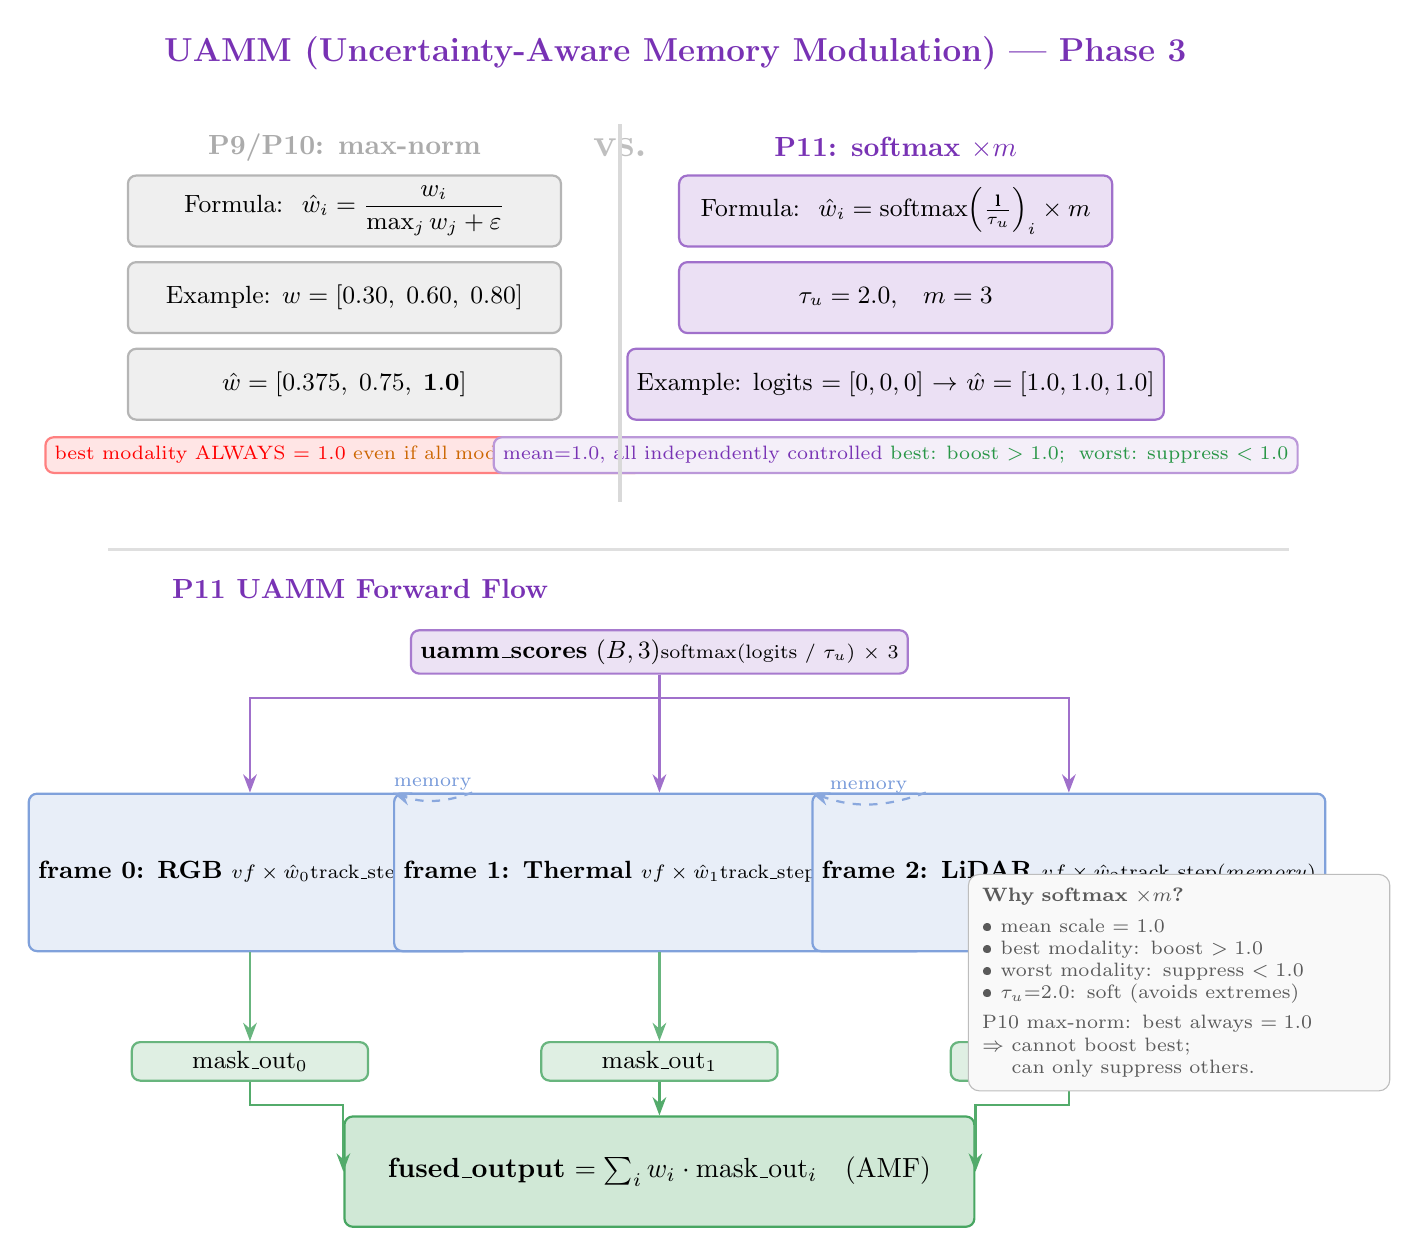
\begin{tikzpicture}

%% ─── Title ───────────────────────────────────────────────────────
\node[font=\large\bfseries, text=cNew] at (7.0, 0.6)
  {UAMM (Uncertainty-Aware Memory Modulation) --- Phase~3};

%% ════════════════════════════════════════════════════════════
%%  TOP: Comparison Panel
%% ════════════════════════════════════════════════════════════
\node[font=\normalsize\bfseries, text=cOld!80] at (2.8,-0.6) {P9/P10: max-norm};
\node[font=\normalsize\bfseries, text=cNew]    at (9.8,-0.6) {P11: softmax $\times m$};
\node[font=\Large\bfseries, text=gray!50]      at (6.3,-0.6) {vs.};

%% max-norm panel
\node[oldB, minimum height=9mm] at (2.8,-1.4)
  {Formula:\; $\hat{w}_i = \dfrac{w_i}{\max_j w_j + \varepsilon}$};
\node[oldB, minimum height=9mm] at (2.8,-2.5)
  {Example: $w=[0.30,\;0.60,\;0.80]$};
\node[oldB, minimum height=9mm] at (2.8,-3.6)
  {$\hat{w}=[0.375,\;0.75,\;\mathbf{1.0}]$};
\node[B, fill=red!10, draw=red!50, minimum width=55mm, font=\scriptsize]
  at (2.8,-4.5)
  {{\color{red}best modality ALWAYS = 1.0}\\[-1pt]
   {\color{orange!80!black}even if all modalities are bad}};

%% softmax x m panel
\node[newB, minimum height=9mm] at (9.8,-1.4)
  {Formula:\; $\hat{w}_i = \mathrm{softmax}\!\left(\tfrac{\mathbf{l}}{\tau_u}\right)_i \times m$};
\node[newB, minimum height=9mm] at (9.8,-2.5)
  {$\tau_u = 2.0$,\quad $m = 3$};
\node[newB, minimum height=9mm] at (9.8,-3.6)
  {Example: logits $=[0,0,0]$ $\to$ $\hat{w}=[1.0,1.0,1.0]$};
\node[B, fill=cNew!8, draw=cNew!50, minimum width=55mm, font=\scriptsize]
  at (9.8,-4.5)
  {{\color{cNew}mean=1.0, all independently controlled}\\[-1pt]
   {\color{cAMF}best: boost $>1.0$;\; worst: suppress $<1.0$}};

%% separator
\draw[gray!30, very thick] (6.3,-0.3)--(6.3,-5.1);

%% ════════════════════════════════════════════════════════════
%%  BOTTOM: P11 Forward Flow
%% ════════════════════════════════════════════════════════════
\draw[gray!25, thick] (-0.2,-5.7)--(14.8,-5.7);
\node[font=\normalsize\bfseries, text=cNew] at (3.0,-6.2)
  {P11 UAMM Forward Flow};

%% uamm_scores from fusion head
\node[wgtB] (US) at (6.8,-7.0)
  {\textbf{uamm\_scores} $(B,3)$\\
   {\scriptsize softmax(logits / $\tau_u$) $\times$ 3}};

%% Three track_step boxes
\node[trackB] (T0) at (1.6,-9.8)
  {\textbf{frame 0: RGB}\\[3pt]
   {\scriptsize $vf \times \hat{w}_0$}\\
   {\scriptsize track\_step(\textbf{init})}};
\node[trackB] (T1) at (6.8,-9.8)
  {\textbf{frame 1: Thermal}\\[3pt]
   {\scriptsize $vf \times \hat{w}_1$}\\
   {\scriptsize track\_step(\textit{memory})}};
\node[trackB] (T2) at (12.0,-9.8)
  {\textbf{frame 2: LiDAR}\\[3pt]
   {\scriptsize $vf \times \hat{w}_2$}\\
   {\scriptsize track\_step(\textit{memory})}};

\draw[A, cNew!70] (US.south)--++(0,-3mm) -| (T0.north);
\draw[A, cNew!70] (US.south)--(T1.north);
\draw[A, cNew!70] (US.south)--++(0,-3mm) -| (T2.north);

%% memory arrows
\draw[Ad, cTrack!60, bend left=20] (T0.north east)
  to node[above, font=\scriptsize, text=cTrack!70]{memory} (T1.north west);
\draw[Ad, cTrack!60, bend left=20] (T1.north east)
  to node[above, font=\scriptsize, text=cTrack!70]{memory} (T2.north west);

%% mask outputs
\node[outB] (O0) at (1.6,-12.2)  {mask\_out$_0$};
\node[outB] (O1) at (6.8,-12.2)  {mask\_out$_1$};
\node[outB] (O2) at (12.0,-12.2) {mask\_out$_2$};

\draw[A, cAMF!70] (T0.south)--(O0.north);
\draw[A, cAMF!70] (T1.south)--(O1.north);
\draw[A, cAMF!70] (T2.south)--(O2.north);

%% AMF fused output
\node[fusB] (FUS) at (6.8,-13.6)
  {\textbf{fused\_output} $= \sum_i w_i \cdot \mathrm{mask\_out}_i$\quad(AMF)};

\draw[A, cAMF!80, thick] (O0.south)--++(0,-3mm) -| (FUS.west);
\draw[A, cAMF!80, thick] (O1.south)--(FUS.north);
\draw[A, cAMF!80, thick] (O2.south)--++(0,-3mm) -| (FUS.east);

%% note
\node[note, text width=50mm] at (13.4,-11.2) {
  \textbf{Why softmax $\times m$?}\\[3pt]
  \textbullet\ mean scale = 1.0\\
  \textbullet\ best modality: boost $>1.0$\\
  \textbullet\ worst modality: suppress $<1.0$\\
  \textbullet\ $\tau_u{=}2.0$: soft (avoids extremes)\\[3pt]
  P10 max-norm: best always $=1.0$\\
  $\Rightarrow$ cannot boost best;\\
  \hphantom{$\Rightarrow$} can only suppress others.
};

\end{tikzpicture}
\end{document}
